\iffalse


%% ------------------------------------------------------------------- %%
\chapter{Introdução}
\label{cap:introducao}

Uma monografia deve ter um capítulo inicial que é a Introdução e um
capítulo final que é a Conclusão. Entre esses dois capítulos poderá
ter uma sequência de capítulos que descrevem o trabalho em detalhes.
Após o capítulo de conclusão, poderá ter apêndices e ao final deverá
ter as referências bibliográficas.


Para a escrita de textos em Ciência da Computação, o livro de Justin Zobel, 
\emph{Writing for Computer Science} \citep{zobel:04} é uma leitura obrigatória. 
O livro \emph{Metodologia de Pesquisa para Ciência da Computação} de 
\citet{waz:09} também merece uma boa lida.

O uso desnecessário de termos em lingua estrangeira deve ser evitado. No entanto,
quando isso for necessário, os termos devem aparecer \emph{em itálico}.

\begin{small}
\begin{verbatim}
Modos de citação:
indesejável: [AF83] introduziu o algoritmo ótimo.
indesejável: (Andrew e Foster, 1983) introduziram o algoritmo ótimo.
certo : Andrew e Foster introduziram o algoritmo ótimo [AF83].
certo : Andrew e Foster introduziram o algoritmo ótimo (Andrew e Foster, 1983).
certo : Andrew e Foster (1983) introduziram o algoritmo ótimo.
\end{verbatim}
\end{small}

Uma prática recomendável na escrita de textos é descrever as legendas das
figuras e tabelas em forma auto-contida: as legendas devem ser razoavelmente
completas, de modo que o leitor possa entender a figura sem ler o texto onde a
figura ou tabela é citada.  

Apresentar os resultados de forma simples, clara e completa é uma tarefa que
requer inspiração. Nesse sentido, o livro de \citet{tufte01:visualDisplay},
\emph{The Visual Display of Quantitative Information}, serve de ajuda na
criação de figuras que permitam entender e interpretar dados/resultados de forma
eficiente.

















%% ------------------------------------------------------------- %%
\chapter{Desenvolvimentos}
\label{cap:desenvolvimentos}

Embora neste exemplo tenhamos apenas um capítulo,  entre a introdução
e a conclusão de uma monografia podemos ter uma sequência de capítulos
descrevendo o trabalho e os resultados. Estes podem descrever
fundamentos, trabalhos relacionados, método/modelo/algoritmo proposto,
experimentos realizados, resulatdos obtidos.

Cada capítulo pode ser organizado em seções, que por sua vez pode
conter subseções. 

Um exemplo de figura está na figura~\ref{fig:graph}.
\begin{figure}[htb]
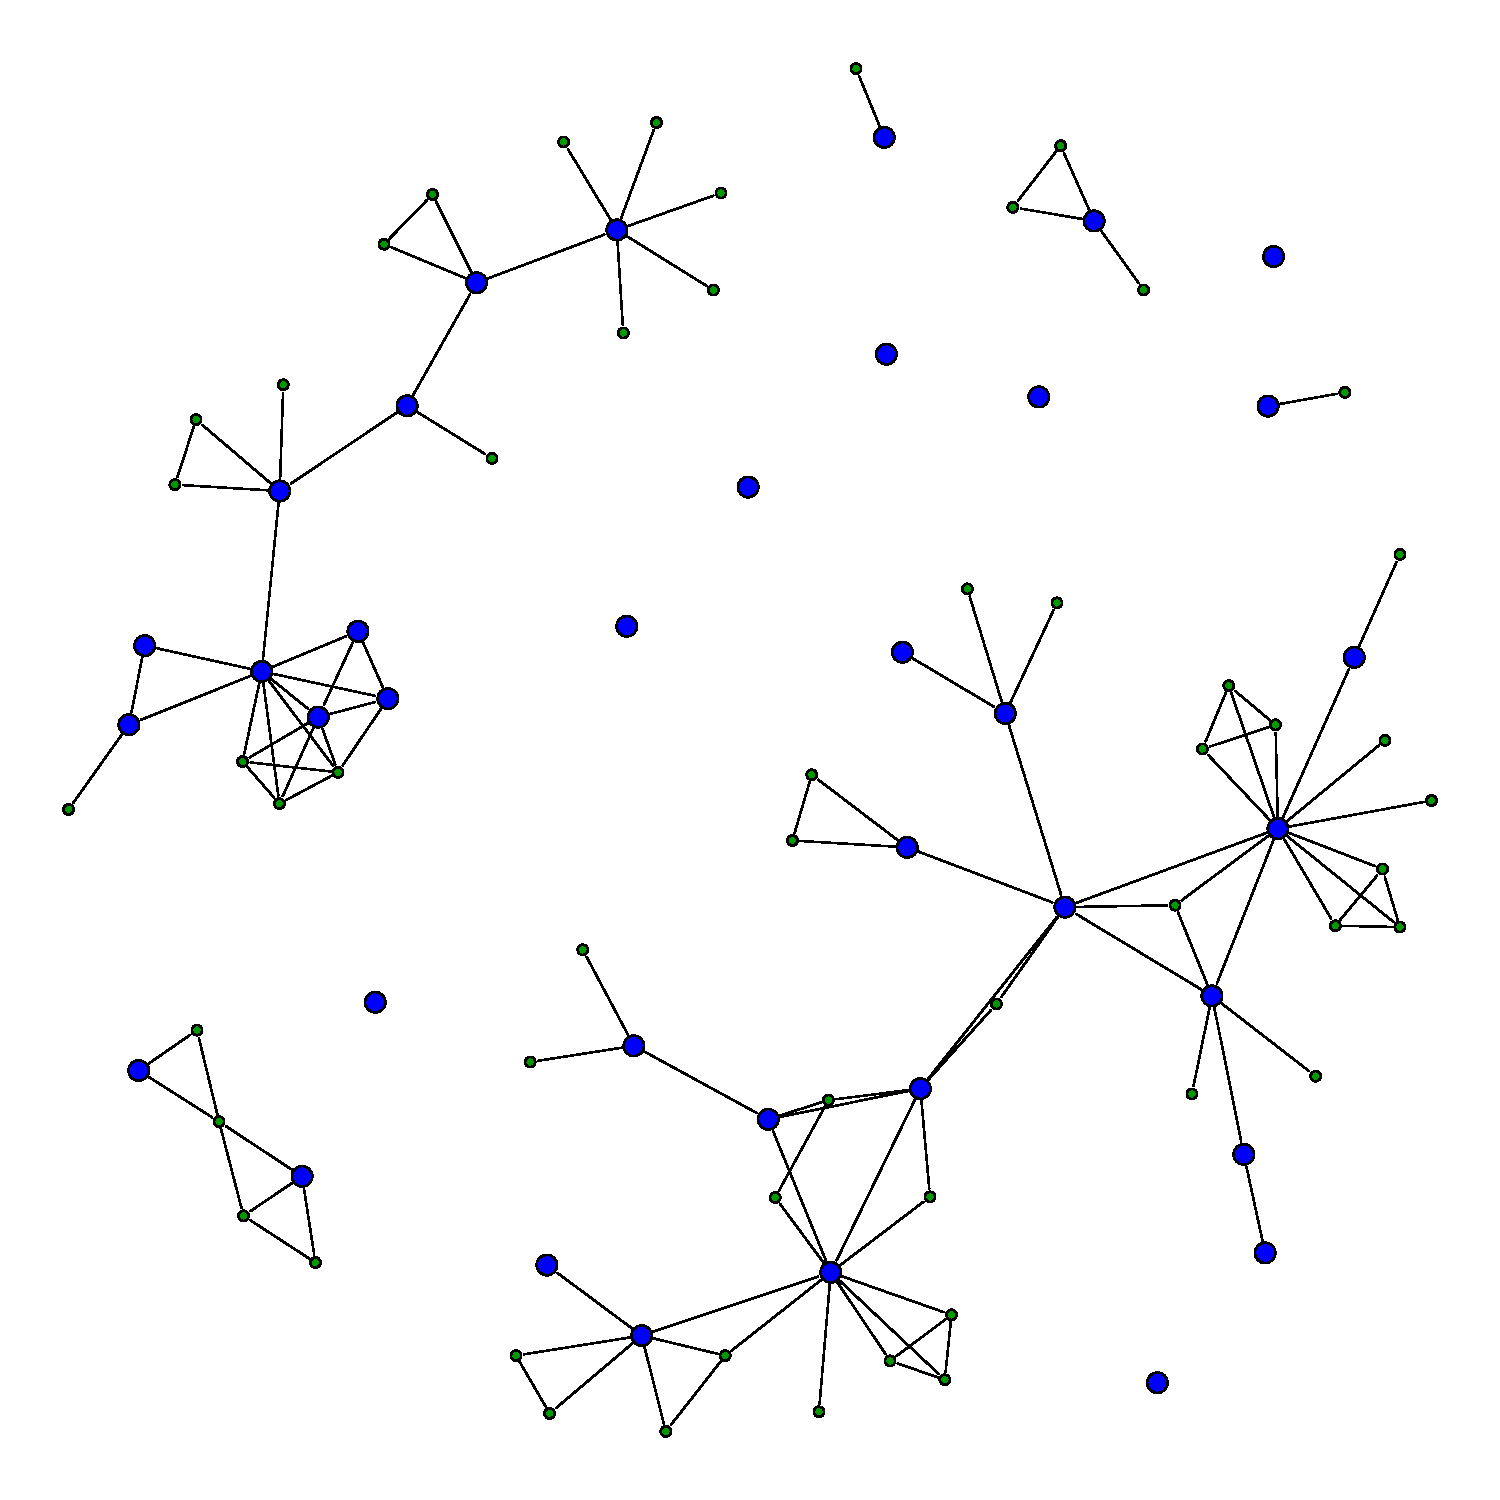
\includegraphics[width=5cm]{figuras/graph}
\caption{\label{fig:graph}Exemplo de uma figura.}
\end{figure}















%% --------------------------------------------------------- %%
\chapter{Conclusões}
\label{cap:conclusoes}

Texto texto texto texto texto texto texto texto texto texto texto texto texto
texto texto texto texto texto texto texto texto texto texto texto texto texto
texto texto texto texto texto texto\footnote{Exemplo de referência para página
Web: \url{www.vision.ime.usp.br/~jmena/stuff/tese-exemplo}}.






\fi